\chapter[Mutation]{Mutation testing}
\label{sec:preliminares.mutation}

\emph{Mutation testing} es un criterio de cobertura que puede ser considerado de \emph{caja blanca}, en donde las metas a cubrir por el test suite, est\'an representadas por fallas artificiales, que deben ser detectadas por el test suite bajo evaluaci\'on. Las fallas artificiales se representan por variantes del programa original, en donde cada una tiene un cambio sint\'actico simple, representando un defecto. Cada variante se denomina \emph{mutante}, mientras que la falla artificial asociada, se llama \emph{mutaci\'on}. Cuantos, de los mutantes generados, son detectados por el test suite, es el valor asociado a este criterio, y se denomina \emph{mutation score}.

Las fallas artificiales utilizadas por este criterio, se agrupan en operadores de mutaci\'on, por ejemplo, el operador de \emph{reemplazo de operadores relacionales} (\emph{ROR}) agrupa las fallas artificiales que cambian un operador relacional en una expresi\'on binaria, por todos los otros disponibles en el lenguaje con el que est\'a escrito el programa.

Como con cualquier criterio, mientras mas cercano al 100\% sea valor asociado, m\'as confianza se puede tener en la calidad del test suite evaluado. En el caso de mutation testing, este valor sube mientras m\'as mutantes sean detectados y baja en caso contrario, sin embargo existen situaciones que afectan de manera negativa a este valor. Ciertas fallas son triviales de detectar, ya sea por que causan que la compilaci\'on o la ejecuci\'on (bajo cualquier entrada) falle, o solo requieren alcanzabilidad para hacerlo, por ejemplo \lstinline|if (c) x = array[-1];|, solo requiere una entrada que satisfaga \emph{c} para detectar la falla, ni siquiera es necesario un or\'aculo para evaluar el resultado. Las fallas triviales aumentan el mutation score sin implicar una mejora en la calidad del test suite. En el espectro opuesto, pueden haber fallas artificiales que tengan el mismo comportamiento sem\'antico, por ejemplo \lstinline|for (int i = 0; i < 10; i++)| es equivalente a \lstinline|for (int i = 0; i < 10; ++i)|. Estos mutantes son llamados equivalentes y por lo tanto indistinguibles del programa original, lo que genera metas que no pueden ser cubiertas, que a su vez disminuye el valor de mutation score, pero el test suite no tiene una peor calidad por no ser capaz de detectar estos mutantes. Finalmente un valor alto de mutation score no significa nada si no existe una relaci\'on entre detectar fallas artificiales y reales.

\section{Propiedades de operadores de mutaci\'on}
\label{sec:preliminares.mutation.opevaluation}

En principio, un operador de mutaci\'on es una funci\'on que aplica a elementos particulares de un programa, ya sea c\'odigo fuente o binarios, y genera versiones modificadas de \'estos. Un operador a su vez deber\'ia tener un objetivo claro, como emular cierto tipo de fallas. Sin embargo para que mutation testing sea un criterio efectivo, algunas propiedades deben ser tenidas en cuenta. \textbf{Tiempo, y otros recursos}, obligan a que el conjunto de mutantes generados se mantenga acotado, de la misma forma en que es necesario acotar el conjunto de tests a utilizar para evaluar un programa. \textbf{Efectividad}, un criterio de cobertura para tests es utilizado para evaluar la calidad de los mismos, precisamente con respecto a cuan efectivos son para detectar potenciales fallas en el programa bajo prueba. Mutation testing tiene un problema similar, dado que la cantidad de fallas artificiales (mutaciones) con las que se va a evaluar a un test suite es finita, genera a su vez, una necesidad de evaluar a \'estos con respecto a su efectividad para evaluar a un test suite para el programa bajo prueba, espec\'ificamente, como el conjunto de mutantes obliga al test suite a ejercitar al programa. \textbf{Representaci\'on de fallas reales}, parece extra\~no que un conjunto de mutantes sea muy efectivo para evaluar un conjunto de tests, pero que no represente fallas reales. Sin embargo, efectividad en la ejercitaci\'on de un test suite solo permite evaluar cuan capaz es \'este de detectar cambios sem\'anticos. Mientras que, una alta efectividad para \'esto, en el contexto de mutantes, no implica que se mantenga para fallas reales, principalmente por que mutation testing intenta emular fallas complejas mediante fallas simples. Un problema ortogonal a estas propiedades, es la confianza, o cuan significativo el valor de mutation score que resulta de un conjunto particular de mutantes. A continuaci\'on vamos a mencionar que cosas afectan o est\'an relacionadas con las propiedades anteriores, y como es posible medirlas.

\subsection{Equivalencia}

Equivalencia [entre dos programas] es una propiedad definida bajo la relaci\'on \texttt{Eq(P, P$\prime$) : $\nexists$ E : P(E) != P$\prime$(E)}, la cual establece que dos programas \texttt{P} y \texttt{P$\prime$} son equivalente si no existe un escenario \texttt{E} tal que el comportamiento de ambos programas sea distinto. Esta es una relaci\'on indecidible, por lo que m\'etodos incompletos son utilizados. Dentro de mutation testing, equivalencia puede encontrarse entre un mutante y el programa original, un caso indeseable ya que \'estos disminuyen el valor del mutation score sin significar una deficiencia de parte del test suite en detectar ciertas fallas artificiales. Otro caso de equivalencia se da entre mutantes, un caso en donde ambos mutantes son detectados por el test suite, sin embargo al ser equivalente incrementan el valor del mutation score sin significar una mejora de parte del test suite en detectar m\'as fallas artificiales.

Dentro de la investigaci\'on sobre la detecci\'on (evaluaci\'on) de esta caracter\'istica y su impacto en el an\'alisis de test suites usando mutation testing, \cite{biblography.mutation.evaluation.equivalent.Schuler+10} propone la utilizaci\'on de diferencia en cobertura de c\'odigo y an\'alisis de fujo de datos para determinar potencial equivalencia. Mientras que  \cite{biblography.mutation.evaluation.equivalent.Just+13} utiliza detecci\'on de restricciones condicionales para alcanzar el c\'odigo mutado y \emph{SAT Solving} para determinar si es posible satisfacer dichas restricciones al tiempo que se obtiene un valor distinto al del programa original en ese punto, lo que es similar en principio a \emph{weak mutation}, en donde se considera que un mutante es detectado si en el estado siguiente a la mutaci\'on se detecta una diferencia con el del programa original, pero a\~nadiendo control de alcanzabilidad y una verificaci\'on exhaustiva acotada para detectar si es posible que exista una diferencia.
En \cite{biblography.mutation.evaluation.equivalent.Grun+09} observan que manualmente, para los casos de estudios utilizados, un programador avanzado tarda aproximadamente 15 minutos en promedio para analizar mutantes equivalentes. Y claramente la existencia de equivalentes disminuye artificialmente el mutation score dando la falsa impresi\'on de que es necesario agregar m\'as tests. Si analizamos el impacto de equivalencia entre mutantes, podemos diferenciar dos casos particulares: equivalencia entre mutantes detectados, \emph{m$_1$} y \emph{m$_2$} son ambos detectados por el test suite bajo evaluaci\'on, sin embargo son equivalentes entre s\'i, esta situaci\'on lleva a un incremento del mutation score por b\'asicamente detectar m\'as de una vez el mismo mutante; equivalencia entre mutantes no detectados, \emph{m$_1$} y \emph{m$_2$} son ambos mutantes sobrevivientes, esto lleva a un decremento del mutation score por b\'asicamente fallar en detectar el mismo mutante dos veces.

\subsection{Dificultad de detecci\'on}

As\'i como los mutantes equivalentes son indeseables por ser imposibles de detectar, los mutantes que son solo detectables por un conjunto peque\~no de tests, son altamente deseables. Estos son denominados \emph{stubborn} \cite{bibliography.mutation.evaluation.stubbornHieronsHD99}. La detecci\'on de estos mutantes requiere tests de ``mejor calidad'', y si bien existen estudios que eval\'uan la generaci\'on de stubborns por operador \cite{bibliography.mutation.evaluation.stubborn}, \'esto depende del conjunto de programas utilizados y los tests asociados. Con respecto a este obst\'aculo, en \cite{bibliography.mutation.evaluation.hardnessVisser}, proponen el uso de \emph{model counting} sobre programas m\'as simples pero utilizando un estudio m\'as exhaustivo. Algunas medidas preventivas para evitar generar mutantes triviales de detectar incluyen controles m\'as estrictos en la generaci\'on, para evitar mutantes que no compilen, por ejemplo, AOIS, un operador que inserta \lstinline|++| y \lstinline|--| en variables aritm\'eticas, puede generar mutantes inv\'alidos si no comprueba que la variable a mutar no es una constante. La raz\'on por la cual detectar o prevenir una baja dificultad de detecci\'on para un conjunto de mutantes, es que es dif\'icil definir precisamente a esta dificultad. Mientras que equivalencia es una propiedad binaria, en el sentido de que, dos programas son o no equivalentes, la dificultad de detecci\'on es una propiedad muy dif\'icil de definir. 

\subsection{Subsunci\'on}

\emph{Subsumption}, la relaci\'on entre mutantes con respecto a los tests que los detectan, da lugar a mutantes redundantes. Esto es, los tests que detectan al mutante subsumido, incluyen a todos aquellos que detectan al que subsume, es decir, el mutante subsumido eval\'ua de manera menos espec\'ifica a los tests, ya que es detectado por una mayor cantidad, mientras que el que subsume eval\'ua tests m\'as espec\'ificos. Esto lleva a mutantes redundantes y representa una forma indirecta de evaluar la dificultad de detecci\'on, los mutantes que subsumen a otros pero no son a su vez subsumidos, son detectados por pocos tests. Presentado inicialmente en \cite{bibliography.mutation.selection.Offutt96}, mutant subsumption es utilizado por \cite{bibliography.mutation.minimizing.dynamicsubsumption} y \cite{bibliography.mutation.evaluation.JustKA17} para evaluar utilidad de mutantes dentro de mutation analysis. Partiendo de que los mutantes utilizados en mutation testing, tienen como objetivo ejercitar a un conjunto de tests para evaluar de manera indirecta la capacidad de los mismos en detectar potenciales fallas reales, aquellos que ejerciten de manera m\'as espec\'ifica a los tests, son considerados entonces, mejores. Un ejemplo de subsuma de mutantes se puede ver en las figuras \ref{figures.examples.subsumptionTable} y \ref{figures.examples.subsumptionGraph}.

\begin{figure}
	\begin{displaymath}
		\begin{array}{llll}
			Tests & M1 & M2 & M3  \\
			1     & \bullet  & \bullet  &     \\
			2     &    & \bullet  & \bullet   \\
			3     &    &    & \bullet  
		\end{array}
	\end{displaymath}
	\caption{Ejemplo de subsuma de mutantes}
	\label{figures.examples.subsumptionTable}
\end{figure}

\begin{figure}
	\begin{center}
		\usetikzlibrary{positioning}
		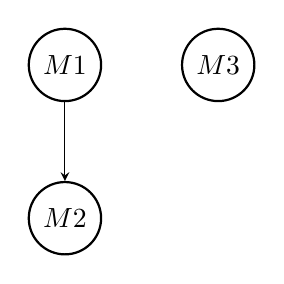
\begin{tikzpicture}[xscale=10, yscale=10,>=stealth]
		\tikzstyle{v}=[circle, minimum size=1mm,draw,thick]
		\node[v] (M1) {$M1$};
		\node[v] (M2) [below=of M1] {$M2$};
		\node[v] (M3) [right=of M1] {$M3$};
		\draw [->] (M1) to (M2);
		\end{tikzpicture}
	\end{center}
	\caption{Grafo de subsuma basado en la Tabla-\ref{figures.examples.subsumptionTable}}
	\label{figures.examples.subsumptionGraph}
\end{figure}

\subsection{Acoplamiento}

\emph{Coupling}, el acoplamiento entre fallas reales y mutantes es una propiedad altamente deseable, sin la misma, mutation testing perder\'ia su utilidad al desaparecer la correlaci\'on entre un mutation score alto y una buena capacidad de parte del test suite para detectar fallas reales. El trabajo m\'as importante sobre este tema, y uno que nos representa una motivaci\'on importante para el desarrollo de nuestro operador de mutaci\'on presentado en esta tesis, es \cite{bibliography.mutation.evaluation.valid-substitute}. El acoplamiento entre mutantes y fallas reales es una relaci\'on que especifica que si un conjunto de tests detecta un conjunto de mutantes, entonces va a detectar una falla real. Por el otro lado, el acoplamiento entre mutantes, representa una situaci\'on indeseable, al ser similar al caso de equivalencia entre mutantes. Una manera si bien poco exigente, para medir acoplamiento entre un programa y un conjunto de mutantes, es evaluar si los tests que detectan las fallas, son los mismos que detectan al conjunto de mutantes. En el trabajo previo, uno de las exigencias adicionales fue solo mutar el c\'odigo asociado a la reparaci\'on de la falla real.

%\section{High order}
%
%\texttt{High Order}, la combinaci\'on de mutaciones, generada al aplicar operadores de mutaci\'on m\'as de una vez al generar un mutante, se denominan mutaciones de alto order mientras que aquellas que la forman, se las llama de primer orden. Si bien en principio esto agregar\'ia una gran cantidad de nuevos mutantes\footnote{Usualmente la cantidad de mutantes al aplicar m\'as de una mutaci\'on por mutante est\'a acotada por M$_0^G$ en donde \texttt{M$_0$} son la cantidad de mutantes de primer orden y \texttt{G} son la cantidad de mutaciones por mutante}, los estudios actuales que se enfocan en esta t\'ecnica concluyen que estos mutantes de alto orden representan fallas artificiales m\'as sutiles y que subsumen a una gran cantidad de mutantes de primer orden. [AGREGAR]